
\index{itk::ImageToImageMetric|textbf}

In ITK, \code{itk::ImageToImageMetric} objects measures quantitively 
how well the transformed moving image fits the fixed image by comparing 
the grayscale intensity of the images. These metrics are very flexible
and can work with any transform or interpolation method and does not
require the reduction of the grayscale images to sparse extracted
information such as edges.

The metric component is perhaps the most critical element of the
registration framework. The selection of which metric to use is highly
dependent on the registration problem to be solved. For example, some metrics
have a large capture range while others require initialization close to
the optimal position; some metrics are only suitable for comparing 
images obtained from the same imaging modality while others can handle
inter-modality comparisions. Unfortunately, there are no clear-cut rules
as to how to choose a metric.

\index{itk::ImageToImageMetric!GetValue()}
\index{itk::ImageToImageMetric!GetDerivatives()}
\index{itk::ImageToImageMetric!GetValueAndDerivatives()}

The basic inputs to a metric are: the fixed and moving images, a
transform and an interpolator. The method \code{GetValue()} can
then be used to evaluate the quantitive criterion at the transform
parameters specified in the argument. Typically, the metric samples 
points within a defined region of the fixed image. 
For each point, the corresponding moving image position is
computed using the transform with the specified parameters, 
then the interpolator is used to compute the moving image intensity 
at the mapped position.

As well as the measure value, gradient-based optimization schemes also require
derivatives of the measure with respect to each transform parameter. The
methods \code{GetDerivatives()} and \code{GetValueAndDerivatives()} can be used
to obtained the gradient information.


Metrics currently available in ITK are:
\begin{itemize}
\item Mean Squares
\item Normalized Correlation
\item Mutual Information
\item Pattern Intensity
\end{itemize}
In the following sections, we describe each metric type in detail. 
For ease of notation, we will refer to the fixed image $f(\bf{X})$ 
and transformed moving image $m \circ T(\bf{X})$ as images $A$ and $B$.

\subsection{Mean Squares Metric}
\label{sec:MeanSquaresMetric}
This metric computes the mean square pixel-wise difference in intensity
between image $A$ and $B$ over a user defined region:

\begin{equation}
MS(A,B) = \frac{1}{N} \sum_i^N \left( A_i - B_i \right)^2
\end{equation}
\begin{center}
$A_i$ is the i-th pixel of Image A\\ 
$B_i$ is the i-th pixel of Image B\\
$N$ is the number of pixels considered
\end{center}

The optimal value of the metric is zero. Poor matches between images
$A$ and $B$ results in large values of the metric. This metric is
simple to compute and have a relatively large capture radius.

This metric relies on the assumption that intensity representing
the same homologous point must be the same in both images. Hence,
its use is restricted to images of the same modality. Additionally,
any linear changes in the intensity result in a poor match value.

\subsection{Normalized Correlation Metric}
\label{sec:NormalizedCorrelationMetric}
This metric computes pixel-wise cross-correlation and normalize it
by the square root of the autocorrelation of the images:

\begin{equation}
NC(A,B) = \frac{ \sum_i^N \left( A_i \cdot B_i \right) }
         { \sqrt { \sum_i^N A_i^2  \cdot \sum_i^N B_i^2 } }
\end{equation}
\begin{center}
$A_i$ is the i-th pixel of Image A\\ 
$B_i$ is the i-th pixel of Image B\\
$N$ is the number of pixels considered
\end{center}

The optimal value of the metric is one. Misalignment between the
images results is small measure values. The use of this metric
is limited to obtained using the same imaging modality. The metric
is insenstive to multiplicative differences between the two
images. This metric produces a cost function with sharp peaks and well
defined maxima. On the other hand, it has a relatively smaller
capture radius.

\subsection{Pattern Intensity Metric}
\label{sec:PatternIntensityMetric}
This metric computes pixel-wise differences and add them 
after passing them through a bell-shaped function $\frac{1}{1+x^2}$:

\begin{equation}
PI(A,B) =  \sum_i^N \frac{ 1 }{ 1 + \lambda \left( A_i - B_i \right) ^ 2 }
\end{equation}
\begin{center}
$A_i$ is the i-th pixel of Image A 
$B_i$ is the i-th pixel of Image B
$N$ is the number of pixels considered
$\lambda$ controls the capture radius
\end{center}

The optimal values is $N$ and poor matches results is small measure
values.

Advantages
\begin{itemize}
\item Produce poor values when few pixels are considered
\item Capture radius can be controled
\item Profile is very pointy (high precision)
\end{itemize}

Disadvantages
\begin{itemize}
\item Limited to same image modality
\item Its derivative is high at the peak this is a problem for some optimizers
\item Sensitive to linear changes in intensity
\end{itemize}


\subsection{Mutual Information Metric}
\label{sec:MutualInformationMetric}
This metric computes the mutual information between image $A$ and image $B$.
Mutual information (MI) measures how much information one random variable
(image intensity in one image) tells about another random variable 
(image intensity in the other image). The major advantage of using
MI is that the actual form of the dependency does not have to be specified. 
Therefore, complex mapping between two images can be modeled. 
This flexibility makes MI well suited as a criterion of multi-modality
registration.

Mutual information is defined in terms of entropy. Let
\begin{equation}
H(A) = - \int p_A(a) \log p_A(a)\, da
\end{equation}
is the entropy of random variable $A$, $H(B)$ entropy of 
random variable $B$ and 
\begin{equation}
H(A,B) = \int p_{AB}(a,b) \log p_{AB}(a,b)\,da\,db
\end{equation}
be the joint entropy of $A$ and $B$.

If $A$ and $B$ are independent then
\begin{equation}
p_{AB}(a,b) = p_A(a) p_B{b}
\end{equation}
and
\begin{equation}
H(A,B) = H(A) + H(B).
\end{equation}
However, if there is any dependency then
\begin{equation}
H(A,B)<H(A)+H(B).
\end{equation}
The difference is called Mutual Information : \( I(A,B) \)
\begin{equation}
I(A,B)=H(A)+H(B)-H(A,B)
\end{equation}

\subsubsection{Parzen Windowing}
In a typical registration problem, direct access to the marginal 
and joint probability densities is not available and hence the
densities must be estimated from the image data. Parzen windows 
(also known as kernel density estimators) can be used for this purpose.
In this scheme, the densities are constructed by taking intensity 
samples $S$ from the image and superpositioning kernel functions 
$K(\cdot)$ centered on the elements of $S$ as illustrated in
Figure \ref{fig:ParzenWindowing}:
\begin{equation}
p(a) \approx P^{*}(a) = \frac{1}{N} \sum_{s_j \in S} K\left(a - s_j\right)
\end{equation}

\begin{figure}
\center
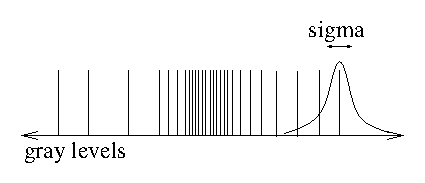
\includegraphics{ParzenWindowing1.eps}
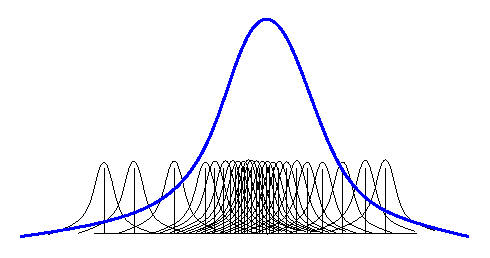
\includegraphics{ParzenWindowing3.eps}
\caption{ In Parzen windowing, a continuous density function is constructed by
superimposing kernel functions (Gaussian function in this case) centered on
the intensity samples obtained from the image. }
\label{fig:ParzenWindowing}
\end{figure}

A variety of functions can be used as the smoothing kernel with the
requirement that it be smooth, symmetric, has zero mean and
integrates to one. For example, boxcar, Gaussian and B-Spline functions.
A smoothing parameter is used to scale the kernel function.
The larger the smoothing parameter, the wider the kernel function
used and hence the smoother the density estimate. If the parameter is
too large, features such as modes in the density will get smoothed out.
On the other hand, if the smoothing parameter is too small, the
resulting density may be too noisy.

The choosing the optimal smoothing parameter is a research 
problem in itself and beyond the scope of this software guide.
Typically, the optimal value of the smoothing parameter will 
depend on the data and the number of samples used.

\subsubsection{Viola and Wells Implementation}
ITK has two mutual information implementation. The first is 
\code{MutualInformationImageToImageMetric} which follows the method specified
by Viola and Wells in \cite{ViolaW:1997}.

\index{itk::MutualInformationImageToImageMetric}

In this implementation, two separate intensity samples $S$ and $R$ are drawn
from the image: the first to compute the density and the second to approximate
the entropy as a sample mean:
\begin{equation}
H(A) = \frac{1}{N} \sum_{r_j \in R} \log P^{*}(r_j).
\end{equation}
Gaussian density is used as smoothing kernel where the standard deviation
$\sigma$ acts as the smoothing parameter.

\index{itk::MutualInformationImageToImageMetric!SetNumberOfSpatialSamples()}

The number of spatial samples used for computation is defined using
method \code{SetNumberOfSpatialSamples()}. Typical values range from 50 to 100.
Note that computation involves an $N \times N$ loop and hence the computation
burden becomes very expensive when a large number of samples is used.

\index{itk::MutualInformationImageToImageMetric!SetFixedImageStandardDeviation()}
\index{itk::MutualInformationImageToImageMetric!SetMovingImageStandardDeviation()}
Quality of the density estimates depends on the choice of the Gaussian kernel
standard deviation. Optimal choice will depend on the content of the images.
In our experiments with the toolkit, we have found that a standard deviation
of 0.4 works well for images which have been normalized to have a mean
of zero and standard deviation of 1.0. The standard deviation of the fixed image
and moving image can be set separatedly using methods 
\code{SetFixedImageStandardDeviation()} and \code{SetMovingImageStandardDeviation()}.

\subsubsection{Mattes et al Implementation}
The second implementation of mutual information is 
\code{MattesMutualInformationImageToImageMetric} which follows the method
specified by Mattes et al in \cite{Mattes:2001}.

\index{itk::MattesMutualInformationImageToImageMetric}
In this implementation, only one set of intensity samples is drawn from the image.
Using this set, the marginal and joint probability density function (PDF)
is evaluated as discrete positions or bins uniformly spread within the dynamic range
of the images. Entropy values are then computed by summing over he bins.

\index{itk::MattesMutualInformationImageToImageMetric!SetNumberOfSpatialSamples()}
\index{itk::MattesMutualInformationImageToImageMetric!SetNumberOfHistogramBins()}

The number of spatial samples used is set using method 
\code{SetNumberOfSpatialSamples()}. The number of bins use to compute
the entropy values is set via \code{SetNumberOfHistogramBins()}.

Since the fixed image PDF does not contribute to the derivatives, it does
not need to be smooth. Hence, a zero order (boxcar) B-Spline kernel is
used for computing the PDF. On the other hand, to ensure smoothness,
a third order B-spline kernel is used to compute the moving image
intensity PDF. The advantage of using a B-spline kernel over a Gaussian kernel
is that the B-spline kernel have a finite support region. This is 
computationally attractive, as each intensity sample only affect a small
of bins and hence does not require a $N \times N$ loop to compute the
metric value.

During the PDF calculations, the image intensity values are linearly to have
a minimum of zero and maximum of one. This rescaling means that a fixed
B-spline kernel bandwidth of one can be used to handle image data 
with arbitrary magnitude and dynamic range.
